\section{The Bigram-Backcopy Task}\label{sec:bb_task}
The Bigram-Backcopy task consists of two sub-tasks: \textit{Bigram-transition} and \textit{Backcopy}. Each input sequence begins with a \bos~token, followed by tokens sampled according to a pre-determined bigram transition probability $\transit$. When some special trigger tokens are encountered, instead of sampling, the preceding token is copied to the next position. Following \citet{bietti2024birth}, we select the transition $\transit$ and the vocabulary $\vocab$ with $| \vocab | = V = 64$ based on the estimated character-level bigram distribution from the tiny \textit{Shakespeare} dataset. In all experiments, the set of trigger tokens $\cT$ is fixed and consists of the $\abs{\cT}=3$ most frequent tokens in the unigram distribution. Thus, the non-trigger token set, $\vocab\setminus \cT$, comprises $61$ tokens.

\subsection{One-layer transformer shows \attnsink s and \valuedrain s.}

On the \bb~task, we pre-train a standard one-layer transformer with only one softmax \attn~head and one \mlp~layer. Unless otherwise specified, the model is trained with Adam for $10,000$ steps.  We relegate the training details in Appendix \ref{sec:ablations}. Figure \ref{fig:bbm-attn} shows that the trained transformer also exhibits the \attnsink~phenomenon, where the \bos~token captures a significant proportion of the attention weights. More importantly, the attention weights reveal interpretable patterns: all non-trigger tokens exhibit \attnsink s, while the attention for trigger tokens is concentrated on their preceding positions. Furthermore, Figure \ref{fig:bbm-value} reveals a value state drain phenomenon similar to LLMs, indicating that on non-trigger tokens, the \attn~head adds a minimal value to the residual stream. 

\begin{figure}[t]
  \centering
  \begin{minipage}{0.38\textwidth}
      \centering
      \subcaption{\small The Bigram-Backcopy task}
      \label{fig:bbm-dgp}
      \vspace{-.2em}
      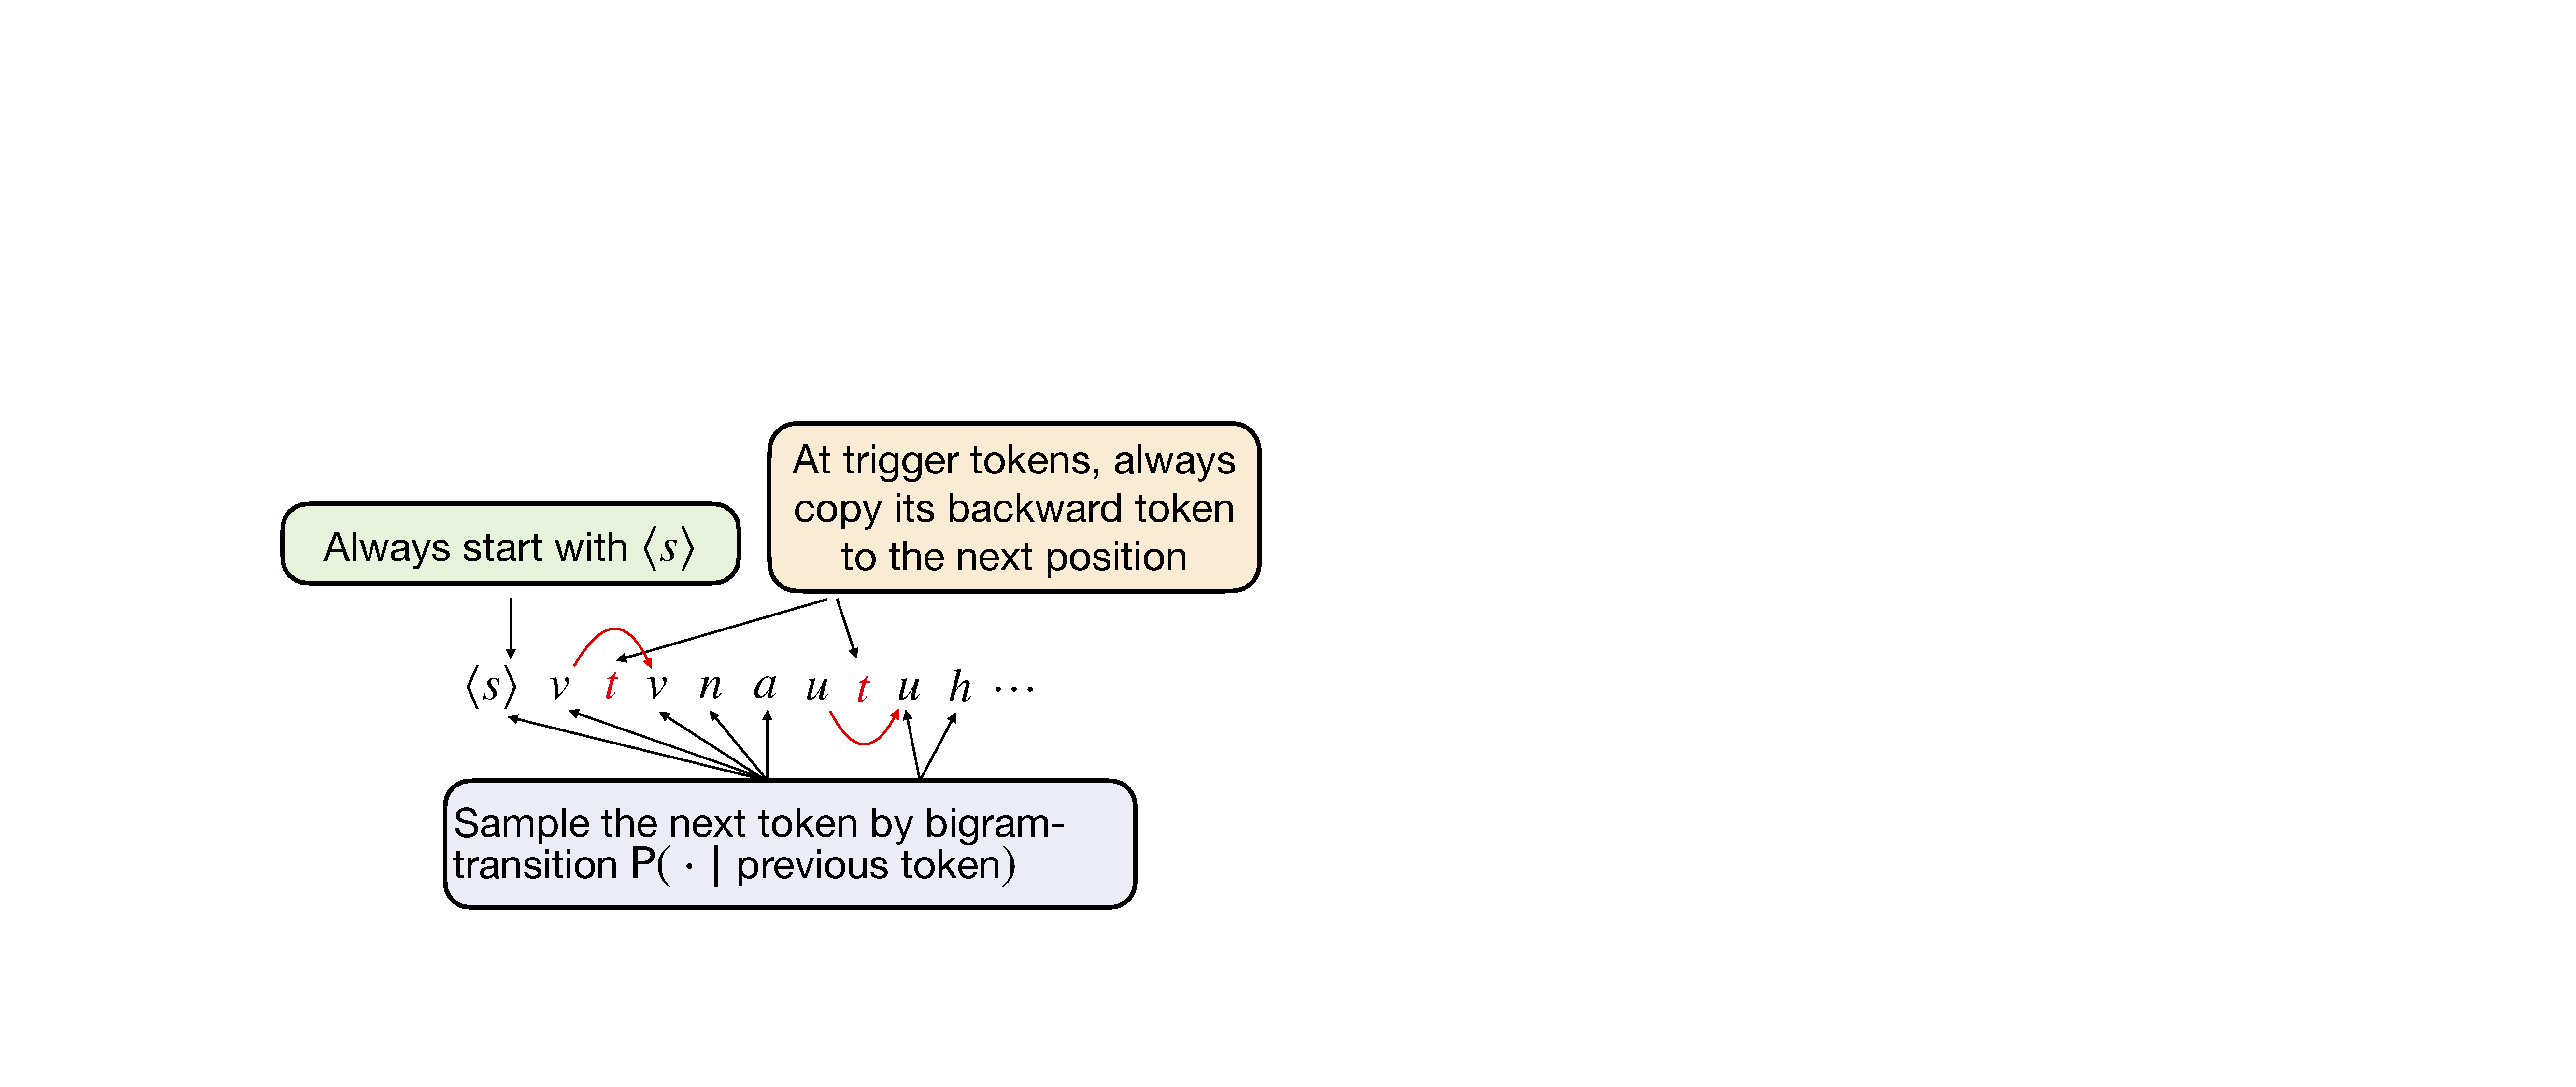
\includegraphics[width=\linewidth]{Figures/BBM/BBM.pdf}
  \end{minipage}
  % \hspace{-1em}
  \begin{minipage}{0.26\textwidth}
      \centering
      \subcaption{\small Attention pattern}
      \label{fig:bbm-attn}
      \vspace{-.2em}
      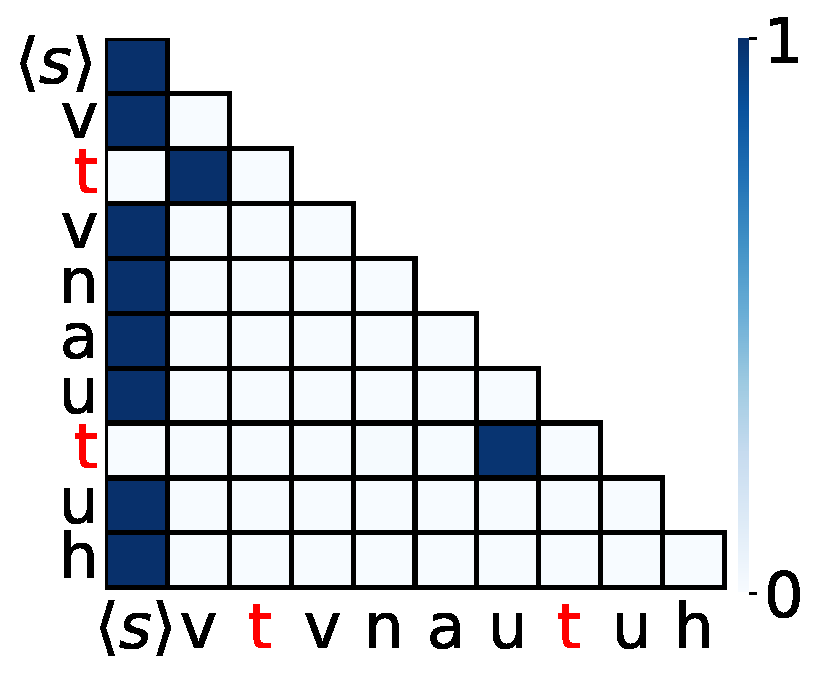
\includegraphics[width=\linewidth]{Figures/BBM/attn_fig1.pdf}
  \end{minipage}
  % \hspace{-1em}
  \begin{minipage}{0.27\textwidth}
      \centering
      \subcaption{\small Small value states}
      \vspace{0pt}
      \label{fig:bbm-value}
      \vspace{-.2em}
      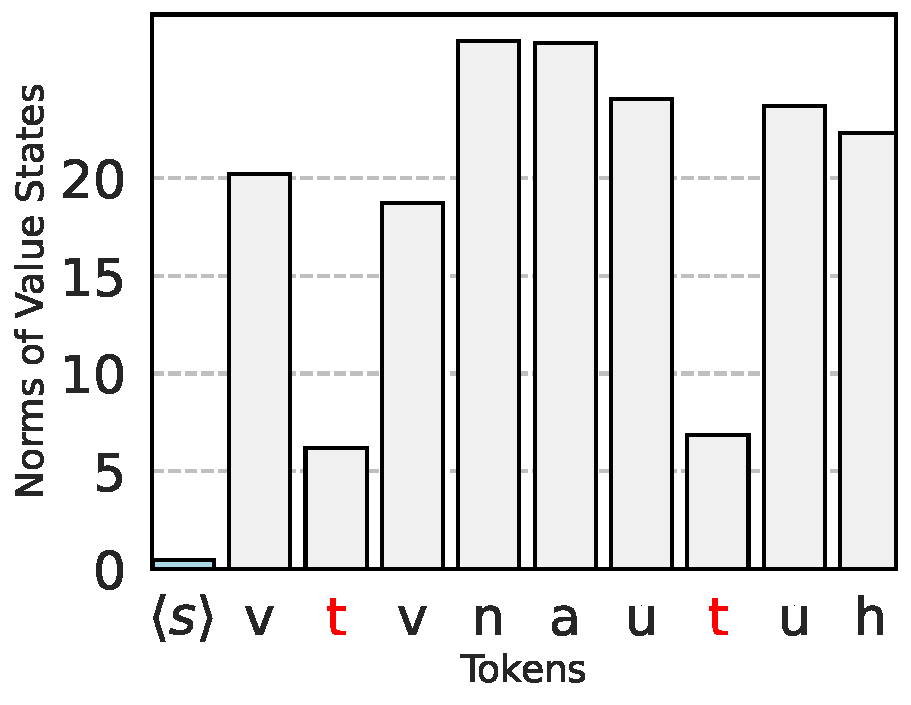
\includegraphics[width=\linewidth]{Figures/BBM/value_states_white.pdf}
  \end{minipage}
  % \vspace{-1em}
  \caption{\small \textbf{Experiments on the Bigram-Backcopy task.} 
  %\sm{Consistently use left (a) instead of reference to self} 
  \textit{Left (a):} We illustrate the data generation procedure for the Bigram-Backcopy task, where we fix 't', 'e', and the space character (' ') as trigger tokens. The BB task samples bigram transitions for non-trigger tokens and backcopies for trigger tokens. \textit{Middle (b):} We present the attention weight heat map of a given prompt, with trigger tokens marked in red. Non-trigger tokens act as attention sinks.  \textit{Right (c):} We plot the value state norms for the prompt, where the \bos~token has a tiny norm.}
  \label{figure:pretraining-findings}
  \vspace{-1em}
\end{figure}

% \begin{figure}[t]
%   \centering
%   \begin{minipage}{0.4\textwidth}
%       \centering
%       \subcaption{\small }
%       \label{fig:pretraining-massive-norm}
%       \vspace{-.2em}
%       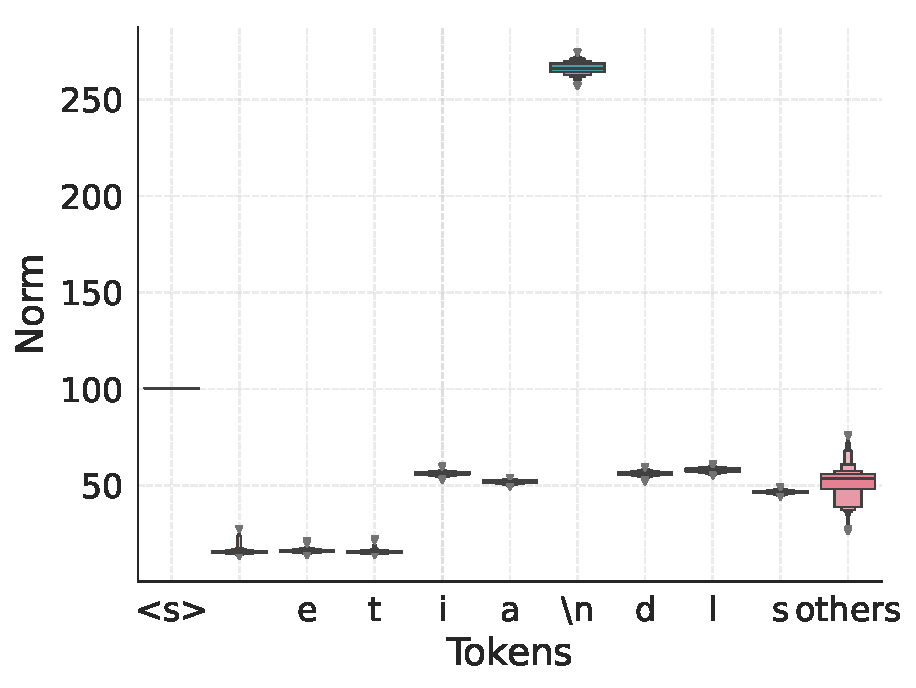
\includegraphics[width=\linewidth]{Figures/figures_pretraining/dormant_copy/dormant_copy_L3_massive.pdf}
%   \end{minipage}
%   \begin{minipage}{0.4\textwidth}
%       \centering
%       \subcaption{\small Small value states norm}
%       \label{fig:pretraining-small-value}
%       \vspace{-.2em}
%       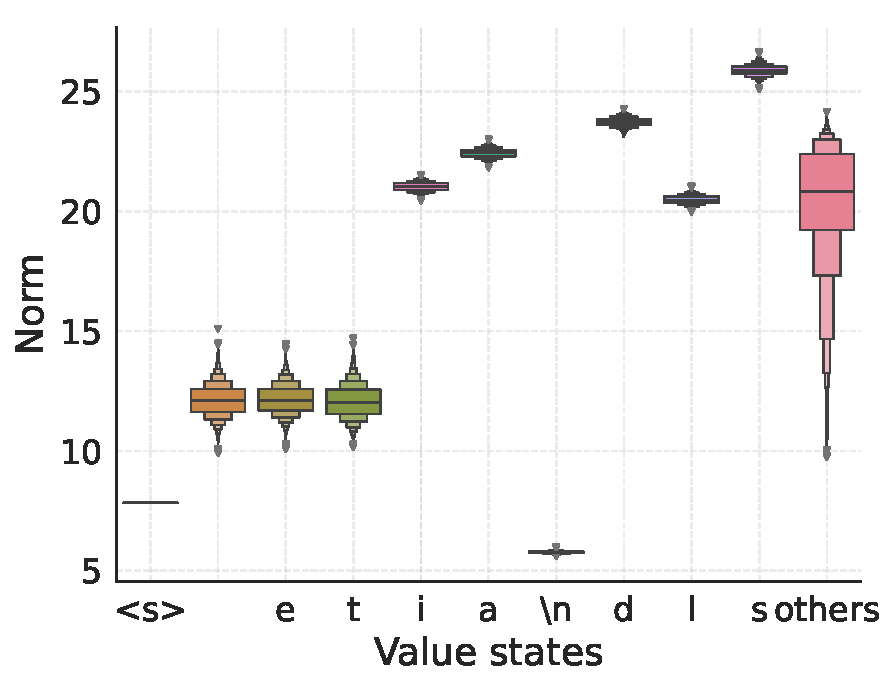
\includegraphics[width=\linewidth]{Figures/figures_pretraining/dormant_copy/dormant_copy_L3_minor.pdf}
%   \end{minipage}
%   \vspace{-1em}
%   \caption{\small \textbf{The norms of residual states and value states in the Bigram-Backcopy task.} A summary of the norm distributions of the output of layer 1 (Figure \ref{fig:pretraining-massive-norm}) and the value states of layer 2 (Figure \ref{fig:pretraining-small-value}) in a 3-layer transformer trained on the \textit{dormant copy} task. The \bos~token is at the left most, with three trigger tokens ` ', `t', and `e' following it. We then randomly choose six tokens and separately summarize their norm distributions. We pull all other tokens together, forming the distribution of the norms of others at the right most. Only the \bos~and the $\backslash n$ token possess remarkably large output norms and small value states norms.}
%   \label{figure:pretraining-findings-norms}
%   \vspace{-1em}
% \end{figure}

\paragraph{The \activedormant~of the attention head:} Inspired by the observed interpretable attention weight patterns, we propose the \textit{\activedormant}. For any given token, an attention head is considered \textit{active} if it contributes significantly to the residual state, and \textit{dormant} if its contribution is minimal. As illustrated in Figure \ref{fig:bbm-attn}, trained on the BB task, the attention head is active on trigger tokens and dormant on non-trigger tokens. 

Figure \ref{fig:interventions} demonstrates that the \mlp~layer is responsible for the Bigram task whereas the \attn~head takes care of the Backcopy task. When the \mlp~layer is zeroed out, the backcopy loss remains significantly better than a random guess, but the bigram loss degrades to near-random levels. Conversely, when the \attn~layer is zeroed out, the backcopy loss becomes worse than a random guess, while the bigram loss remains unaffected. This suggests that on trigger tokens, the \attn~head is active and handles the backcopy task, whereas on non-trigger tokens, the \attn~head is dormant, allowing the \mlp~layer to handle the Bigram task. We summarize the \activedormant~of the \attn~head in Claim \ref{claim:active-dormant}.

\begin{claim}
\label{claim:active-dormant}
In the BB task, the \attn~head demonstrates \activedormant, alternating between two phases:
\begin{itemize}[leftmargin=2em]
\setlength\itemsep{0pt}
\item \textbf{Dormant phase}: On non-trigger tokens, the \attn~head puts dominant weights to the \bos~token, adding minimal value to the residual stream, having little impact on the model’s output.
\item \textbf{Active phase}: On trigger tokens, the \attn~head puts dominant weights to the relevant context tokens, adding substantial value states to the residual stream, resulting in a significant impact on the model’s output. 
\end{itemize}
\end{claim}

\paragraph{The growth of attention logits on the \bos~token and the decrease in the norm of its value state.} Figure \ref{fig:dynamics} displays the training dynamics of excess risks, attention weights, attention logits, and value state norms for the \bos~token. All values are rescaled to highlight the trends. The backcopy excess risk and the bigram excess risk both drop to zero within the first 1000 steps. As the backcopy risk decreases, the attention weights on the \bos~token increase, suggesting a relationship between the formation of attention sinks and the functional development of the attention heads. For each token $\tok_n$ at position $n$ in the prompt, we compute $\text{logit}_{\bos} = \mathtt{mean}_{n}[\langle \query_{\tok_n}, \key_\bos \rangle - \mathtt{mean}_{i}(\langle \query_{\tok_n}, \key_{\tok_\toki}) \rangle]$, which serves as a progress measure for attention sinks. Even after the attention weights on the \bos~token is nearly $1$, $\text{logit}_{\bos}$ continues to increase. Simultaneously, the norm of the value state of the \bos~token continues to decrease to a small value.

\begin{figure}
  \centering
  \begin{minipage}{0.37\textwidth}
      \centering
      \subcaption{\small Excess risk after interventions}
      \label{fig:interventions}
      % \vspace{-0.5cm}
      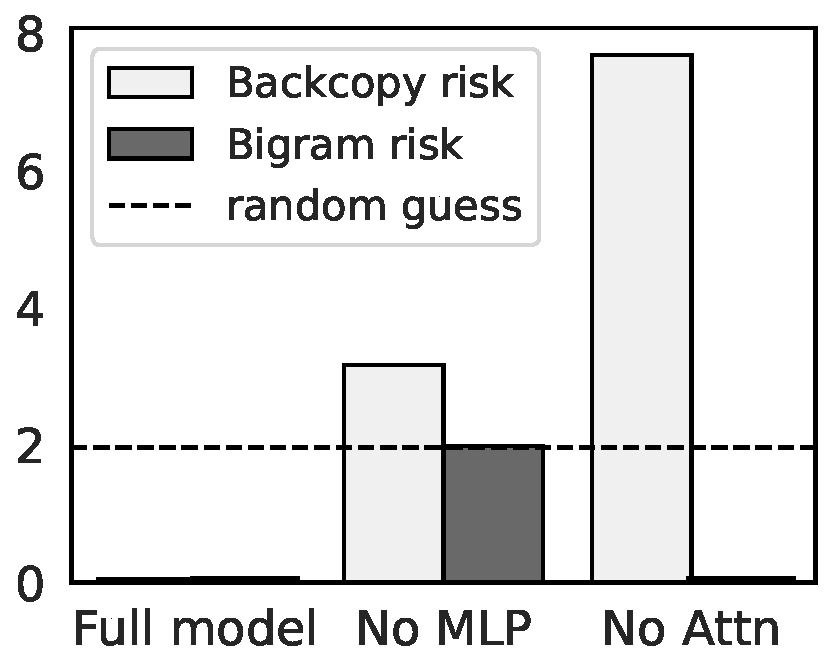
\includegraphics[width=\textwidth]{Figures/BBM/interventions.pdf}
  \end{minipage}
  % \hspace{1em}
  \begin{minipage}{0.6\textwidth}
      \centering
      \subcaption{\small Training dynamics }
      \label{fig:dynamics}
    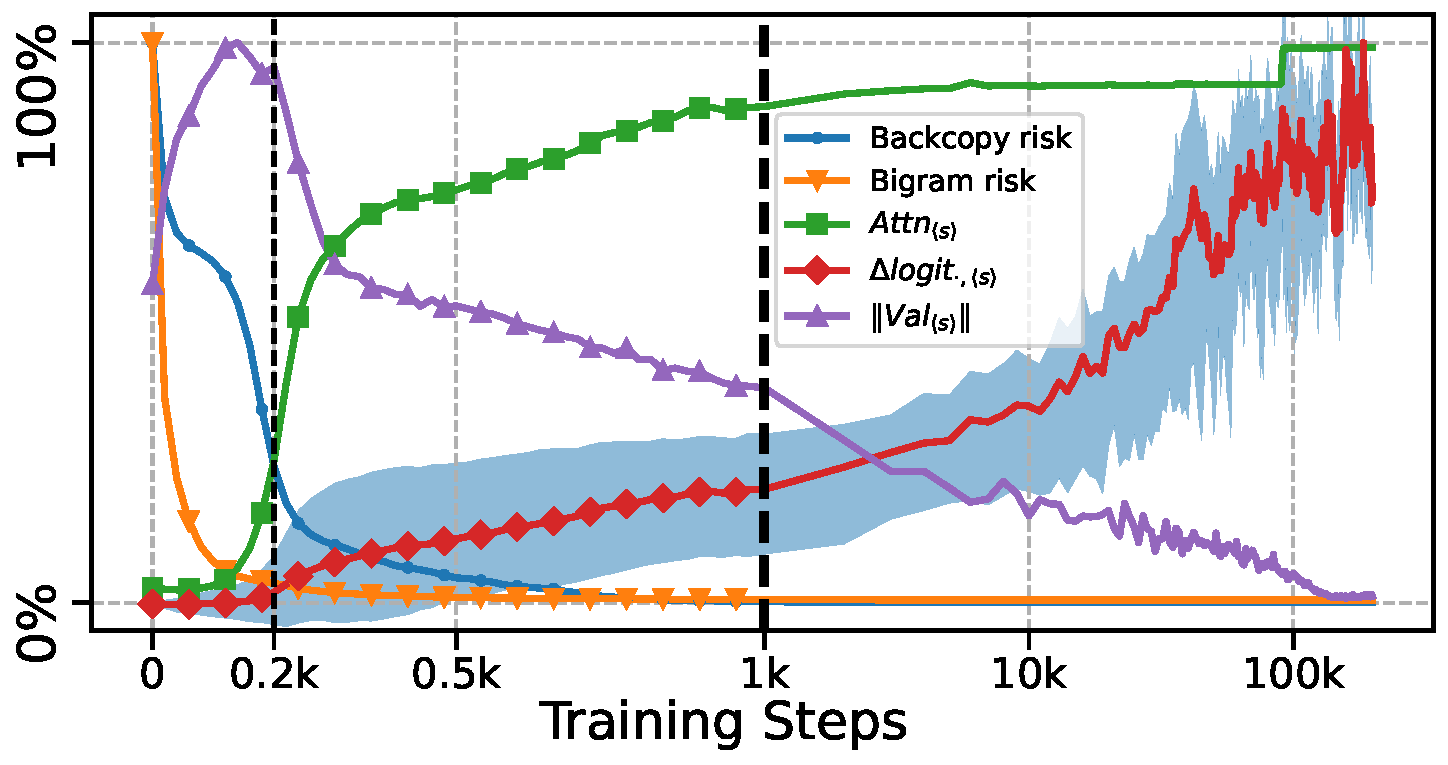
\includegraphics[width=\textwidth]{Figures/BBM/dynamics_combine.pdf}
  \end{minipage}
  \hspace{-1em}
    \caption{\small \textbf{Interventions and dynamics of one-layer transformer on the Bigram-Backcopy task.}  \textit{Left (a)}: We display the excess risks for a one-layer model trained on the Bigram-Backcopy (BB) task under various interventions. \textit{Right (b):} We plot the excess risks, attention weights, attention logits, and value state norms for the \bos~token along the training dynamics. Each curve is rescaled to fall within a 0 to 1 range, though the trends remain consistent without rescaling. On the right side of \textit{(b)}, the horizontal axis is logarithmically scaled. The $\text{logit}_{\bos}$ curve denotes the mean of attention logits from all given non-trigger query tokens $\tok$ on the \bos~token, normalized by the mean of attention logits on other tokens. The shaded area gives the 90\% confidence interval on the distribution over all non-trigger tokens.}
    \label{figure:verify-assumptions}
\end{figure}

\subsection{Analysis of a minimally-sufficient transformer architecture}

\begin{figure}[t]
    \centering
    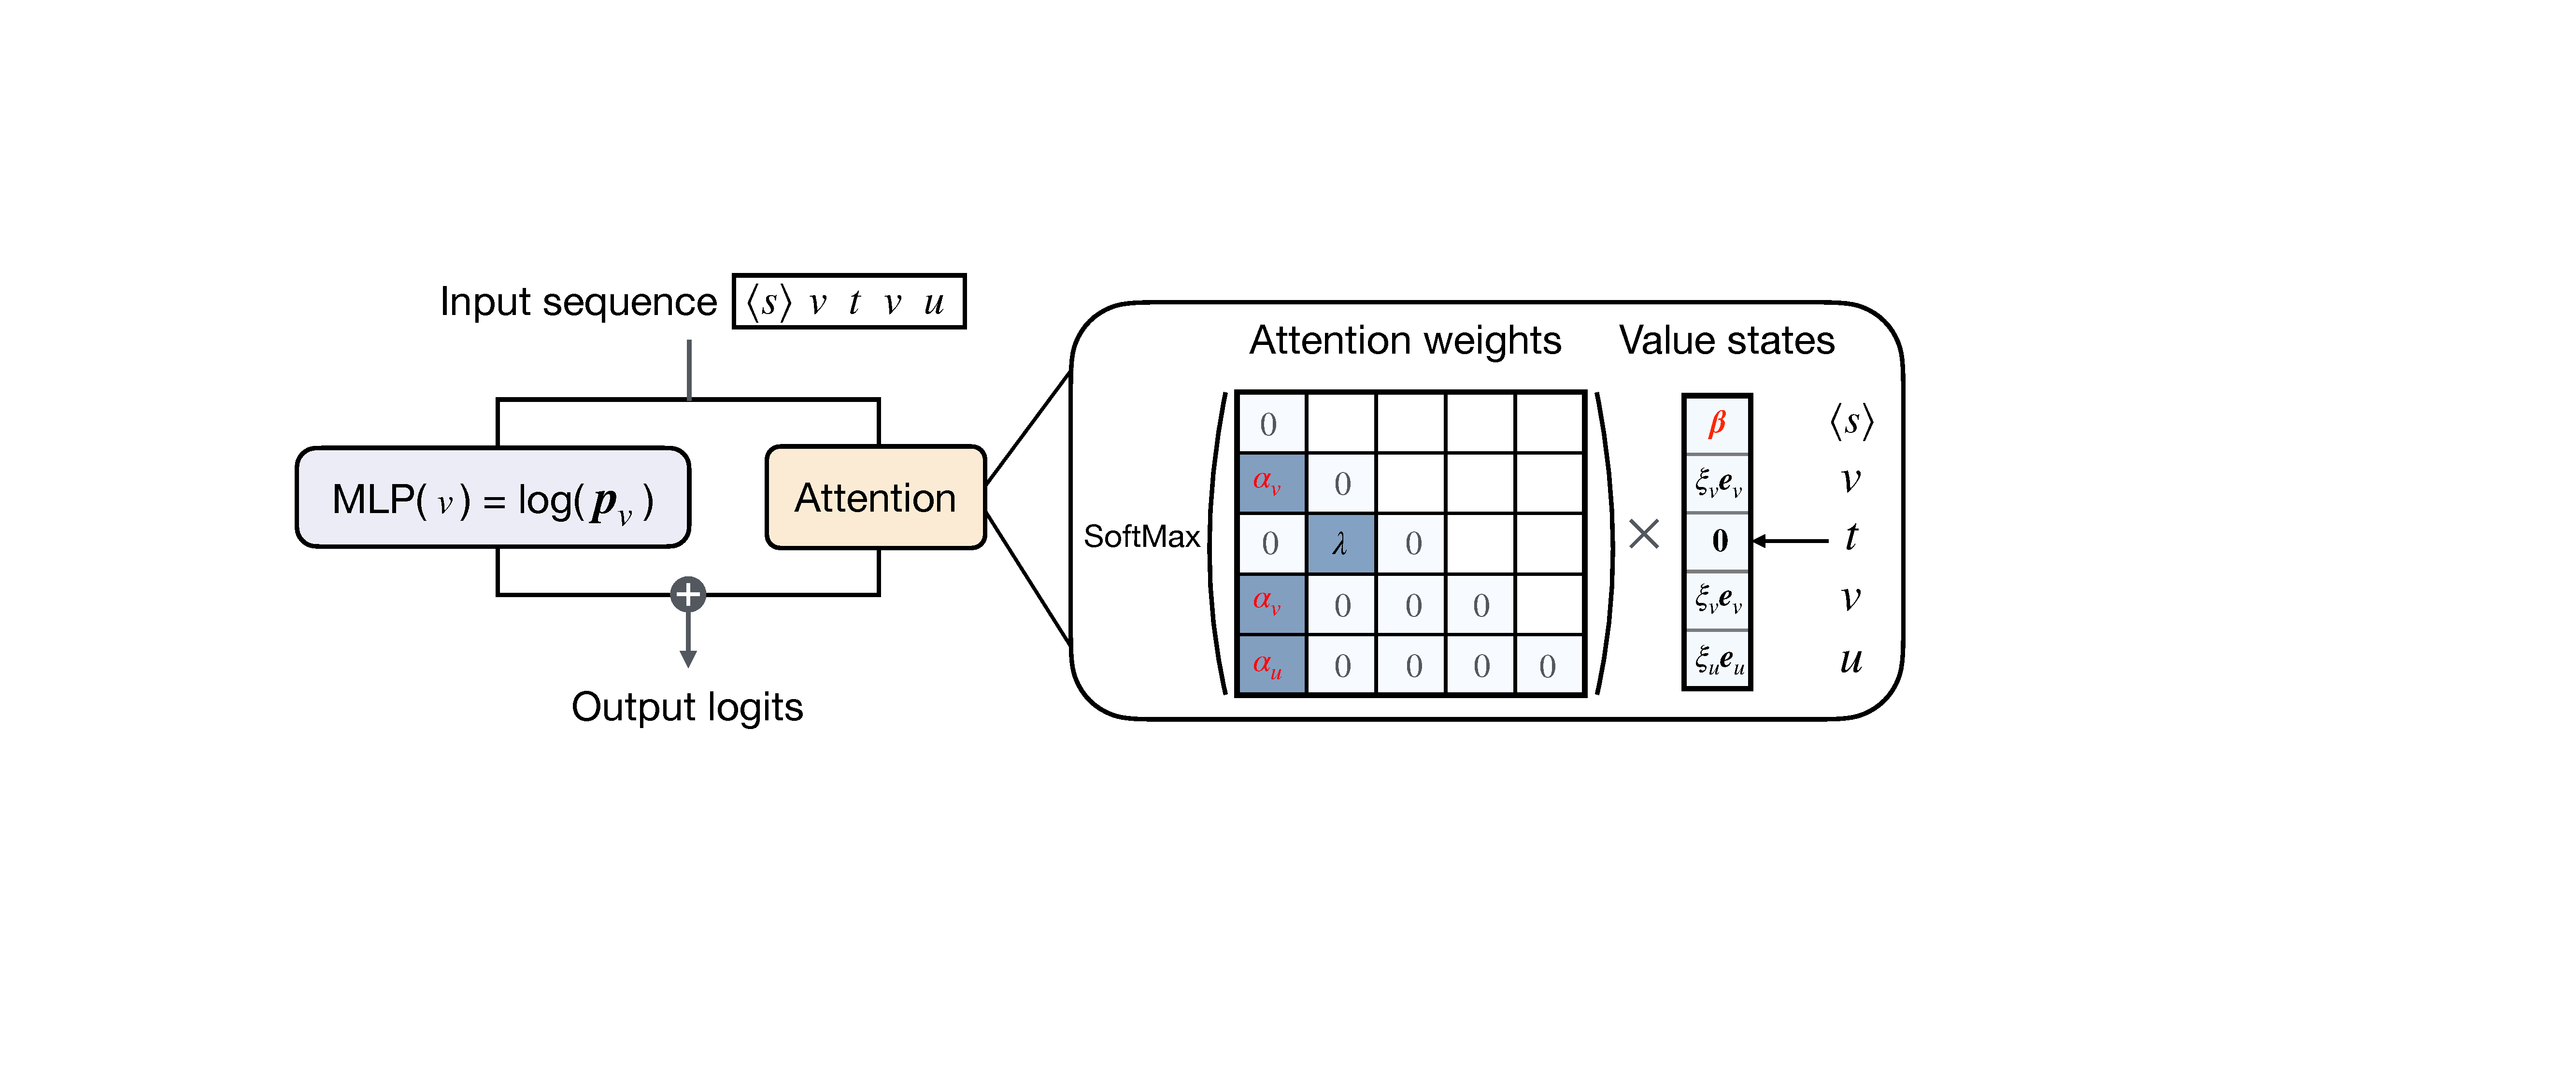
\includegraphics[width=0.8\linewidth]{Figures/BBM/SimpleModel.pdf}
    \caption{\small \textbf{The simplified transformer architecture with one \mlp-layer and one \attn~head in parallel.} The predicted probability is the softmax of the output. Assume that the trainable variables are $(\vecsink,\vecvalue) \in \R^V \times \R^V$, which stands for the attention logits and value states of the $\bos$ tokens.}
    \label{figure:simple-model}
\end{figure}

In this section, we analyze the training dynamics on the BB task by simplifying the architecture while preserving the attention sinks and value state drains phenomena. Let $\vocab$ denote the set of all tokens except the $\bos$ token, and $\cT$ denote the set of all trigger tokens. Given any $\tok \in \vocab$, we denote $\transition_{\tok\tokk}=\transit(\tokk|\tok)$ to be the next token Markov transition probability, and $\bp_v = [p_{v1}, \ldots, p_{vV}]$ be the row vector in the simplex. We assume that the tokens are embedded into $V$-dimensional space using one-hot encoding, and for notation simplicity, we abuse $v$ to stand for its one-hot encoding vector $\bm{e}_v \in \R^V$ which is a row vector. The predicted probability of the $n+1$ token is given by $\softmax(\TF([\bos; v_{1:n-1}; v])_n)$, where transformer architecture is given by $\TF(\cdot) = \attn(\cdot ) + \mlp(\cdot )$. Here $\attn(\cdot ) = \softmax(\mask(\query(\cdot ) \key(\cdot )^\top )) \vall(\cdot )$ and $(\query, \key, \vall)$ are linear maps from $\R^V \to \R^V$. Since the \mlp~layer could handle the Bigram task, we assume that $\mlp$ outputs the Markov transition probabilities $\bp_v$ on non-trigger tokens $v$ and zero on trigger tokens. For the \attn~head, we assume that the attention logits on the $\bos$ key-token are $(\sink_{v_1}; \ldots; \sink_{v_n})$, the attention logits on any trigger query-token are $(0, \ldots, \lambda, 0)$ where the second last coordinate is $\lambda$, and assume other logits are zero. Assume that the value state of $\bos$ is $\vecvalue \in \R^V$, and the value state of each non-trigger token $\tok$ is a one-hot encoding vector $\bm{e}_\tok$ multiplied by $\xi_\tok \geq 0$. Figure \ref{figure:simple-model} illustrates this simplified transformer architecture. These assumptions are summarized in the following equations. 
\begin{equation}\label{eqn:simplification_TF}
\begin{aligned}
&~ \mlp(\tok) = \log \bp_v \cdot 1\{ \tok \not\in \cT  \} ~~~ \text{for } \tok \in \vocab,\\
&~\langle \query(\tok), \key(\bos) \rangle =\sink_\tok \cdot 1 \{ v \not\in \cT \}~~~\text{for } \tok\in\vocab, \\
&~\langle \query(\tok), \key(\tok') \rangle = \lambda \cdot 1\{ \tok \in \cT, \tok' \text{ is the former token of } \tok \} ~~~\text{for } \tok, \tok' \in \cV, \\
&~ \vall(\tok) = \xi_\tok \bm{e}_\tok  ~~~\text{with $\xi_\tok=0$ for $\tok\in\cT$, and $\xi_\tok\geq 0$ for $\tok\in\vocab\setminus\cT$.}
\end{aligned}
\end{equation}

Theorem \ref{thm:construction} demonstrates the existence of a transformer structure that is equivalent to the simplified version. We relegate the proof in Section \ref{sec:proof}.

\begin{theorem}\label{thm:construction}
For any parameters $(\vecsink \in \R^{V}, \vecvalue \in \R^V, \bm{\xi} \in \R^V, \lambda \in \R)$, there is a one-layer transformer $(\mlp, \query, \key, \vall)$ such that Eq. (\ref{eqn:simplification_TF}) holds. The transformer gives ground truth transition of the BB model if $\min_{v \in \vocab} \sink_v \to\infty$, $\min_{v \in \vocab} \xi_v \to\infty$, $\lambda\to \infty$, and $\vecvalue=0$.
\end{theorem}

% \sm{I am here.} We make further simplifications on the loss function. Given a non-trigger token at position $n$, assume $W=\sum_{i=1}^n \exp \query_n^\top \key_i $. Assume that $W=\sum_{\tokk=1}^\vocabsize W_\tokk$, with each $W_\tokk$ corresponds to the summations from . We assume that they are fixed values and do not depend on the position $n$. %In reality $W\approx N/2$, which is half of the total sequence length. Since token $\tokk$ takes a proportion $\stable_\tokk$ in the stable distribution, $W_\tokk \approx \stable_\tokk W$ on average. 
Throughout we adopt Eq.~(\ref{eqn:simplification_TF}) as our assumption. We further define $W_{\tokk} = \sum_{i = 1}^n 1\{ \tok_i = \tokk \}$, $\bm{W} = (W_1, \ldots, W_V)$, and $W = \sum_{\tokk \in \vocab} W_{\tokk} = n$. Then for a non-trigger token $v$, the output of attention layer with input sequence $[\bos; v_{1:n-1}; v]$ gives (denoting $\xi_{\tokk} = 0$ for $\tokk \in \cT$)
\[
\TF([\bos; v_{1:n-1}; v])_n = \log \bp_v + \frac{e^{\sink_\tok}}{e^{\sink_\tok} + W} \vecvalue + \sum_{\tokk=1}^{\vocabsize} \frac{W_\tokk \xi_\tokk}{e^{\sink_\tok} + W} \cdot \bm{e}_\tokk.
\]
% Combining the above simplifications, we get that
% \[
% \TF([v_{1:n-1}; v])=\Big[\log \transition_{\tok1} + \frac{e^{\sink_\tok}\ivalue_1+W_1\xi_1}{e^{\sink_\tok}+W};\ldots;\log \transition_{\tok\vocabsize} + \frac{e^{\sink_\tok} \ivalue_\vocabsize+W_\vocabsize\xi_\vocabsize}{e^{\sink_\tok}+W}\Big].
% \]
Therefore, on the non-trigger token $\tok$, the cross-entropy loss between the true Markov transition $\bp_\tok$ and predicted transition $\softmax(\TF([\tok_{1:n-1}; \tok])_n)$ is given by
\[
\loss_\tok(\sink_\tok, \vecvalue) = \sum_{\tokk=1}^\vocabsize \transition_{\tok\tokk}\Big\{ \log \Big[ \sum_{\toki=1}^\vocabsize \transition_{\tok\toki} \exp\Big(\frac{e^{\sink_\tok}\ivalue_\toki+W_\toki\xi_\toki}{e^{\sink_\tok}+W}\Big) \Big] - \frac{e^{\sink_\tok}\ivalue_\tokk+W_\tokk\xi_\tokk}{e^{\sink_\tok}+W} - \log \transition_{\tok\tokk} \Big\}.
\]
For simplicity, we neglect the loss on trigger tokens and assume that $(\{ W_i \}_{i \in [V]}, W)$ are fixed across different positions in the input sequences\footnote{We note that \cite{reddy2023mechanistic} makes similar simplification in analyzing induction heads.}, and consider the total loss to be the losses on each non-trigger token averaged with its proportion in the stable distribution $\{\pi_v\}_{v \in \vocab}$, given by
\[
\loss(\vecsink,\vecvalue) = \sum_{\tok \in \vocab \setminus \cT} \stable_\tok \loss_\tok(\sink_\tok, \vecvalue).
\]
% \tianyu{change the summation notation in the proof.}
\begin{theorem}\label{thm:main}
Consider the gradient flow of the loss function $\loss(\vecsink, \vecvalue)$. Assume $\xi_\tok \ge 0$ for any $\tok$, and $\{ W_i \cdot \xi_i \}_{i \in \vocab}$ are not all equal. 
\begin{itemize}[leftmargin=2em]
\setlength\itemsep{0pt}
    \item (Attention logits grow logarithmically reinforced by small value states) Fix $\vecvalue= \beta \cdot \bm{1}$ for a constant $\beta$, and consider the gradient flow over $\vecsink$. With any initial value $\vecsink(0)$, there exists $\bm{r}(t)$ with norm uniformly bounded in time such that 
    \[\vecsink(t) = \frac{1}{2} \log t \cdot \bm{1} + \bm{r}(t).\]
    \item (Value state shrinks to a small constant vector reinforced by large attention logits) Fix $\vecsink = \sink \cdot \bm{1}$ for a constant $\sink$, and define $\bar{\ivalue}(0) = V^\inv[\sum_{\tok} \ivalue_\tok(0)]$. Consider the gradient flow over $\vecvalue$. As $t \to \infty$, we have
    \[\vecvalue(t) \to \vecvalue^\star = \bar\ivalue(0) \cdot \bm{1} - e^{-\sink} \cdot \bm{W}\circ \bm{\xi}.\]
    \item (Stable phase: identical attention logits) Consider the gradient flow over variables $(\vecsink, \vecvalue)$. Any vector of the following form
    \[\vecsink = \sink \cdot \bm{1}, \quad \vecvalue = c \cdot \bm{1} - e^{-\sink} \cdot \bm{W} \circ \bm{\xi},  ~~~ \sink, c\in\R \]
     is a stationary point. These are all global minimizers of $\loss(\vecsink,\vecvalue)$.
\end{itemize}
\end{theorem}
The proof of Theorem~\ref{thm:main} is provided in Appendix~\ref{app:proof-main}. We give three key remarks: (1) As $\sink_\tok\to\infty$, a Taylor expansion of the gradient $\partial \loss/\partial \sink_\tok$ suggests that $\mathrm{d}\sink_\tok/\mathrm{d}t \propto \exp(-2 \sink_\tok)$, which leads to the logarithmic growth of $\sink_\tok$. Similar logarithmic growth exists in the literature under different setups \citep{tian2023scan,han2023lm}. (2) For a fixed $\vecsink=\sink\bm{1}$, under additional assumptions on the initial value $\vecvalue(0)$, we can prove a linear convergence for $\vecvalue$. (3) The stable phase described in Theorem \ref{thm:main} seems to imply that the system could be stable without attention sinks, as it does not require $\sink$ to be large. However, in practice, models trained on the BB task tend to converge to a stable phase where $\sink$ is relatively large. 
% \tianyu{We expect LLMs to converge to the stable phase outlined in Theorem \ref{thm:main} as well.}
% Revisiting Figure \ref{fig:attention_logits_random}, which shows attention logits in Llama 2-7B, the attention logits on the \bos~token appear identical. 
% Thus, we expect LLMs to converge to the stable phase outlined in Theorem \ref{thm:main} as well.

\paragraph{The Formation of Attention Sinks and Value State Drains.} When $\vecvalue = \bm{0}$, the attention logits on the \bos~token increase monotonically. This demonstrates that the presence of a small value state of the \bos~token reinforces the formation of attention sinks. When $\vecsink = \sink \cdot \bm{1}$, with $\sink$ sufficiently large, $\vecvalue(t) \to \bar{\ivalue}(0) \bm{1}$. Given the random Gaussian initialization, $\|\bar{\ivalue}(0) \bm{1}\|_2 \approx \|\vecvalue(0)\|_2 / \sqrt{d}$, where $d$ is the hidden dimension. This demonstrates that the presence of attention sinks reinforces the formation of value states drains.

% \paragraph{combine to the previous paragraph} Although all the $\vecsink=\sink \bm{1}$, $\vecvalue=c\bm{1}-e^{-\sink} \bm{W}\circ \bm{\xi}$ are stable phases. Only the phase with $\vecsink\to \infty$ and $\vecvalue\to c \bm{1}$ can match the oracle algorithm with any out of distribution input. When the value $\sink$ is finite, $\vecvalue$ depends on the value $\bm{W}\approx \bm{\stable} W$, which strongly depends on the stable distribution $\bm{\stable}$. Therefore, if tested with OOD input that has different stable distribution, it cannot match the oracle algorithm.

\paragraph{Experimental verification.} Revisiting Figure \ref{fig:dynamics}, which shows the dynamics of a full transformer model trained with Adam, we observe that both $\text{logit}_{\bos}$ and $\|\vall_{\bos}\|_2$ exhibit growth rates consistent with Theorem \ref{thm:main}. The $\text{logit}_{\bos}$ is equivalent to $\sink$ in this context, as all other attention logits are assumed to be zero under the setup of Theorem \ref{thm:main}. When plotted on a logarithmic scale, the $\text{logit}_{\bos}$ curve grows approximately linearly between 1,000 and 10,000 steps, then accelerates before stabilizing around 100,000 steps.  Meanwhile, the norm of the value state decreases monotonically. The simultaneous increase in attention weights and decrease in value-state norms suggest that these phases occur together during the training process. To further validate Theorem \ref{thm:main}, we construct a simplified model that aligns with Equ. \eqref{eqn:simplification_TF}, and train the parameters $(\vecsink \in \R^{V}, \vecvalue \in \R^V, \bm{\xi} \in \R^V, \lambda \in \R)$ with Adam. The resulting training curves are similar to those of a one-layer transformer, also exhibiting the mutual reinforcement mechanism.

Combining theoretical insights and experimental evidence, we summarize the formation of attention sinks and value state drains as a mutual reinforcement mechanism.

% P = f(X, V_1, V_2) (ground truth). When P is independent of V_1, V_2, f(X, V_1, V_2) = f(X); Assume p = f(x, 0, 0). Now we fit it with p = f(x, a_1 v_1, a_2 v_2). When v_1, v_2 \neq 0, we need to have a_1, a_2 = 0 to make accurate prediction. 

\begin{claim}[Mutual reinforcement mechanism]
For any attention head given a specific prompt, if the model can accurately predict the next token without the attention head, but adding any value state from previous tokens worsens the prediction, the attention head becomes dormant, forming an attention sink, leading to the mutual reinforcement of attention sinks and value state drains: 
\begin{enumerate}[leftmargin=2em]
\setlength\itemsep{0pt}
    \item The SoftMax mechanism pushes the attention weights to the value state drains, reinforcing attention sinks.
    \item The attention sinks on the value state drains further pushes down the value state, reinforcing value state drains.
    % \item The value state drains attract more attention weights, reinforcing the attention sinks.
\end{enumerate} 
The mutual reinforcement stabilizes at the phase when all tokens have identical large attention logits on the value state drains. 
%\sm{This sentence appears here seems weird} \tianyu{I added mutual reinforcement mech}
Finally, due to the causal mask, the training dynamics favor the \bos~token to become an extreme token.
\end{claim}

We expect that the formation of extreme tokens in LLMs follows a similar mutual reinforcement mechanism. Indeed, although Theorem \ref{thm:main} focuses on a specific BB task with a simplified architecture and loss function, the same principles can be applied to more general scenarios. Specifically, for an attention head $\attn$, we assume that $(\text{LLM}\setminus \attn)(\tok) = \log \bm{\transition}_\tok$, meaning that the LLM, even if we zeroed out  $\attn$, can still output an accurate next token prediction. Furthermore, we assume $\val(\tok) = \xi_\tok \bm{e}_\tok$, indicating that adding the value state from any previous tokens performs a specific function. Under these assumptions, we expect the same theoretical results to apply to LLMs. In Section \ref{sec:llm}, we will explore the formation of attention sinks and value state drains along the training dynamics of LLMs, where we find empirical evidence that aligns with the theory. 

\begin{figure}
  \centering
    \begin{minipage}{0.3\textwidth}
      \centering
      \subcaption{\small ReLU attention}
      \label{fig:relu-attn}
      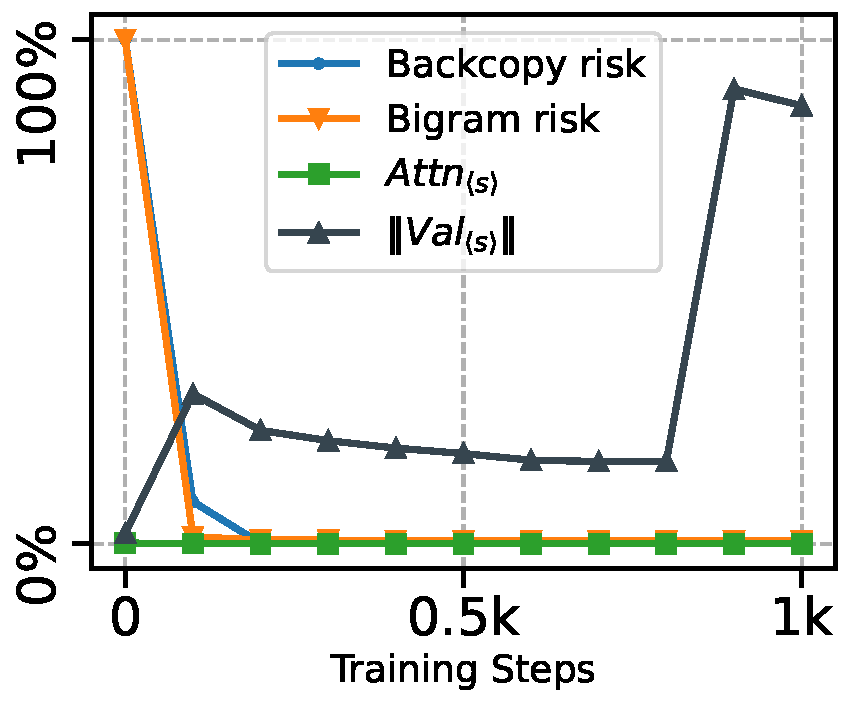
\includegraphics[width=\textwidth]{Figures/BBM/relu_dynamics.pdf}
  \end{minipage}
    \begin{minipage}{0.33\textwidth}
      \centering
      \subcaption{\small Interventions on a 3-layer TF}
      \label{fig:massive-interventions}
      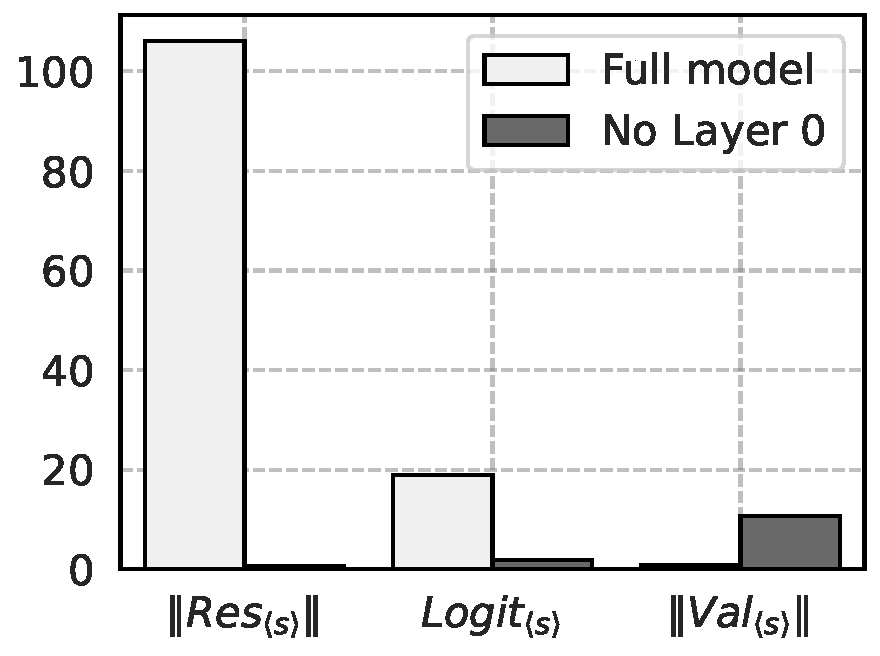
\includegraphics[width=\textwidth]{Figures/BBM/massive_interventions.pdf}
  \end{minipage}
  \begin{minipage}{0.33\textwidth}
      \centering
      \subcaption{\small Eliminating
      residual state peaks}
      \label{fig:sgd}
      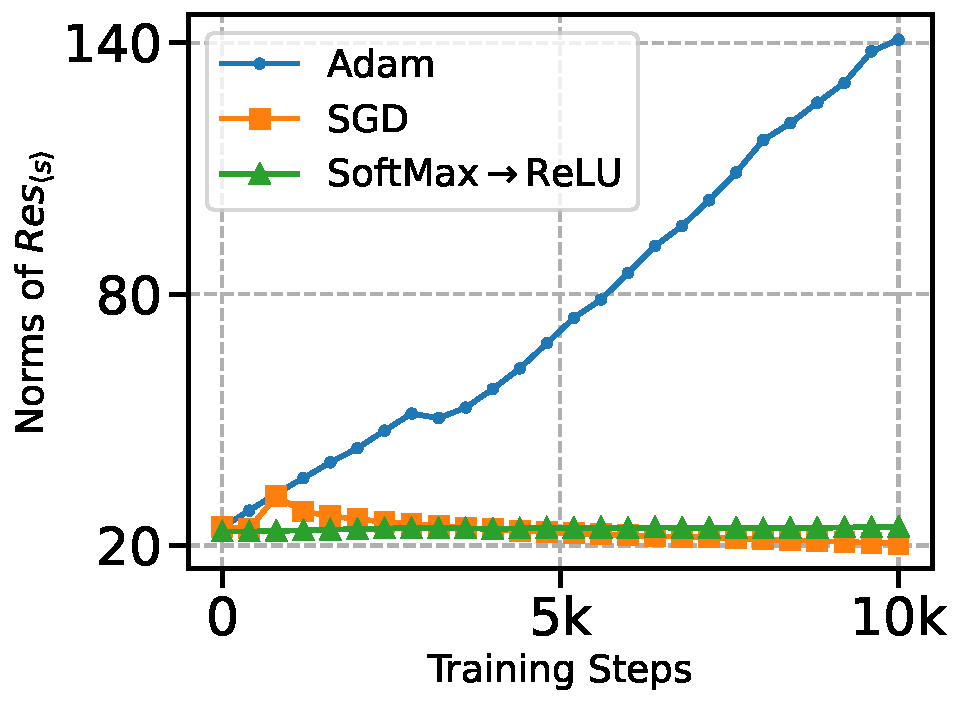
\includegraphics[width=\textwidth]{Figures/BBM/adam_vs_sgd.pdf}
  \end{minipage}
    \caption{\small \textbf{Experiments on massive norms with multi-layer transformers trained on the Bigram-Backcopy task.} 
    \textit{Left (a):} We present the training dynamics of the ReLU attention for the first 1,000 steps.
    \textit{Middle (b):} We plot the intervention results on the \attn+\mlp+\attn+\mlp+\mlp~structure.
    % Figure \ref{fig:minimal-massive} \sm{no self reference in caption} shows the  $\|\Output(\bos)\|_2$ at layer 0 across different model architectures. 
    \textit{Right (c):} We plot the evolution of massive norms in a three-layer transformer trained with Adam, SGD, and using a ReLU attention structure. Notably, only the three-layer model with softmax attention trained using Adam results in the emergence of residual state peaks. \sm{Figure (c) y label $Res_{<s>}$}\tianyu{looks fine to me?}}
\end{figure}

\paragraph{Replacing SoftMax by ReLU attention removes extreme-token phenomena.} As an implication of our theory, we predict that training with ReLU attention instead of SoftMax attention will eliminate the extreme-token phenomena. Without the SoftMax, the dynamics no longer push the attention weights on the \bos~token, which remains zero along the training dynamics. Without attention sink, the dynamics no longer push down the value state norm, and the mutual reinforcement mechanism breaks. Figure~\ref{fig:relu-attn} illustrates the training experiment on the BB task replacing SoftMax with ReLU, showing that both the Bigram and Backcopy risk match the Bayes risk after 200 training steps, but the attention logits of \bos~do not grow, and the value state does not shrink, confirming the prediction. 

\subsection{The emergence of residual state peaks}
\paragraph{The residual state peaks require a three-layer structure.}  No residual state peaks appear in a one-layer transformer trained on the BB task. We train various models on the BB task and track the \bos~token’s residual state norms after layer $0$. We relegate the experimental results to Appendix \ref{sec:ablations}. We find that a three-layer transformer is enough to produce residual state peaks. 
% In Figure \ref{fig:minimal-massive},  
If we allow to skip some \mlp~or \attn~layers, the ``\attn+\mlp+\attn+\mlp+\mlp'' combination becomes the simplest model that produces residual state peaks (Figure \ref{appfigure:massive_minimal}). Circuit analysis also reveals that LLMs typically add a large vector in the first layer and cancel it in the last layer. We propose that the add-then-cancel mechanism is essential for residual state peaks and requires at least three layers.

\paragraph{Residual state peak reinforces attention sinks and value state drains in trained models.} Figure \ref{fig:massive-interventions} presents the intervention results on the ```\attn+\mlp+\attn+\mlp+\mlp'' model. We recenter the $\|\res_{\bos}\|_2$ by subtracting the average norm of other tokens from the \bos~token norm. The $\text{logit}_{\bos}$ and $\|\val_{\bos}\|$ are computed in layer $1$ following the same ways as in Figure \ref{fig:dynamics}. When layer 0 is zeroed out, the residual norm returns to normal, attention logits decrease, and the value state norm rises. It verifies that the residual state peak contributes to the attention sink and value state drain phenomenon in the trained transformer.

% \paragraph{I plan to put the theory for residual state peaks part in the appendix} To include the 
% To model the dynamics of massive norms, we assume that $\cos(\query_i, \key_0)=1$ for any $i$. The output of the lower layer adds $m \key_0/\ltwo{\key_0}$ on the residual stream of the \bos~token and get $\bh_0+m\key_0$. Assume that $\ltwo{\bh}=1$ and $\cos(\bh, \key_0) = c$. As a result,  

% \paragraph{Conjecture: The \activedormant~and the use of Adam reinforce the linear growth of residual state peaks in dynamics.} Since residual state peaks drive attention sinks and value state drains in trained transformers, we hypothesize that the \activedormant~strengthens their formation. Specifically, when the training dynamics push the attention logits on the \bos~token, it also pushes up the norm of $\attn_0(\bos)$ and $\mlp_0(\bos)$ in layer 0. Due to the layer norm, their gradients shrink quickly, but Adam makes small gradients to be constant updates. Further experiments support the conjecture. Figure \ref{fig:sgd} shows the \bos's residual state norms after layer $0$ of three-layer transformers with different configurations. Adam leads to a linear increase in residual norms. In contrast, with SGD, attention sinks persist, but residual state peaks vanish. The ReLU attention, which lacks the \activedormant, shows no residual peaks. 

\tianyu{I want to keep parts of the original explanations.}
\paragraph{Replacing Adam by SGD removes the linear growth of residual state norm.} Figure \ref{fig:sgd} shows the \bos's residual state norms at the output of layer $0$ of three-layer transformers with different configurations. Adam leads to a linear increase in residual norms. In contrast, with SGD, attention sinks persist, but residual state peaks vanish. The ReLU attention, which lacks the \activedormant, shows no residual state peaks. 
% Therefore, we hypothesize that the \activedormant~strengthens their formation. Specifically, when the training dynamics push the attention logits on the \bos~token, it also pushes up the norm of $\vall_{\bos}$ and $\mlp_{\bos}$ in layer 0. Due to the layer norm, their gradients shrink quickly, but Adam makes small gradients constant updates, leading to a linear increase in residual norms.


% \begin{itemize}
%     \item The attention sinks and value state drains are external manifestations of the active-dormant mechanism in LLMs.
%     \item The attention heads go through the attention-increasing and value-state-shrinking phases. They converge to the stable phase with identical attention logits on the \bos~token.
%     \item The residual state peaks reinforce attention sinks and value state drains. Both the lower layer attentions and MLPs contribute to the residual state peaks.
%     \item The residual states go through linear increasing phase in the pre-training.
% \end{itemize}


% \subsection{Verify the predictions from the theory}



